

%template setup, made it adhere to UWA standards
\documentclass[12pt, a4paper]{article}
\usepackage{graphicx}
\usepackage{amsmath}
\setlength{\oddsidemargin}{0.5cm}
\setlength{\evensidemargin}{0.5cm}
\setlength{\topmargin}{-1.6cm}
\setlength{\leftmargin}{0.5cm}
\setlength{\rightmargin}{0.5cm}
\setlength{\textheight}{24.00cm} 
\setlength{\textwidth}{15.00cm}
\parindent 0pt
\parskip 5pt
\pagestyle{plain}


%meta info
\title{CITS4008 Assignment 2: Beyond the Thermodynamic Hypothesis}
\author{Max Ward}
%let the date get auto generated

%author list formatter. not really needed here, but always nice to have
\newcommand{\namelistlabel}[1]{\mbox{#1}\hfil}
\newenvironment{namelist}[1]{%1
\begin{list}{}
    {
        \let\makelabel\namelistlabel
        \settowidth{\labelwidth}{#1}
        \setlength{\leftmargin}{1.1\labelwidth}
    }
  }{%1
\end{list}}



%-------------------------------------------------------------------------

\begin{document}


%title first!
\maketitle

\begin{abstract}
The algorithmic prediction of RNA molecules dates back to the late 1970s. Despite the fields age, little progress has been made. There are two core approach to in silico RNA folding: ad-hoc dynamic programming algorithms, and stochastic context free grammar parsing methods. Both converge on the same accuracy upper limit, despite often using wildly different scoring schemes. In this report I outline these core algorithmic approach to folding RNA. Furthermore I highlight the lack of progress in prediction accuracy. Finally I attempt to explain why, and suggest a direction for future research.
\end{abstract}

\tableofcontents
\clearpage

%assignment is too small to require numbered sections, or chapters
\section*{Introduction} 
Ribonucleic Acid (RNA) is a biologically active molecule similar in structure to DNA. Recent research has found myriad functions for RNA. For example, RNA can act as a catalyst for mRNA splicing, peptide bond formation, and can alter the regulation of genes
\cite{xu2012statistical}. Because of its inherently single stranded nature, RNA forms bonds with itself, folding into
secondary and tertiary structures \cite{conn1998rna}.

It is axiomatic that chemical structure is tantamount to biological function, and RNA is no exception. For this reason, there has and continues to be an intense
interest in predicting the secondary structure of RNA
molecules in silico. This is  because it will allow the detection and classification of unknown RNAs, and assist the design of new RNA based drugs \cite{condon2003problems}. The secondary structure of RNA
is also highly conserved during evolution, indicating its importance \cite{hofacker2008rna}.

I endeavour to give the reader a brisk but incisive review of RNA secondary structure prediction algorithms in this paper. For the sake of succinctness, my focus shall be pseudoknot-free RNA prediction methods, particularly those able to predict RNA structures ex nihilo---that is with no information other than the RNA sequence itself.

\section{Dynamic Programming}
\subsection{The Nussinov Algorithm}
According to the `Thermodynamic Hypothesis', biologically active molecules should form structures that have minimal free energy and thus maximum stability \cite{anfinsen1973principles}. For RNA molecules, counting bonds is a crude but nonetheless accurate measure of energetic stability, as every bond increases the
stability of a structure \cite{nussinov1978algorithms}. In the late 1970s, when the first large RNA molecules
were being successfully sequenced, Nussinov et al. \cite{nussinov1978algorithms} introduced an algorithm to find a single structure with maximal number of bonds using dynamic programming. This is possible only with the restriction that all bonding pairs are nested, and hence contains no pseudoknots.

\begin{figure}
\begin{center}
%the image is quite large, needs to be scaled dwon
\scalebox{0.3}{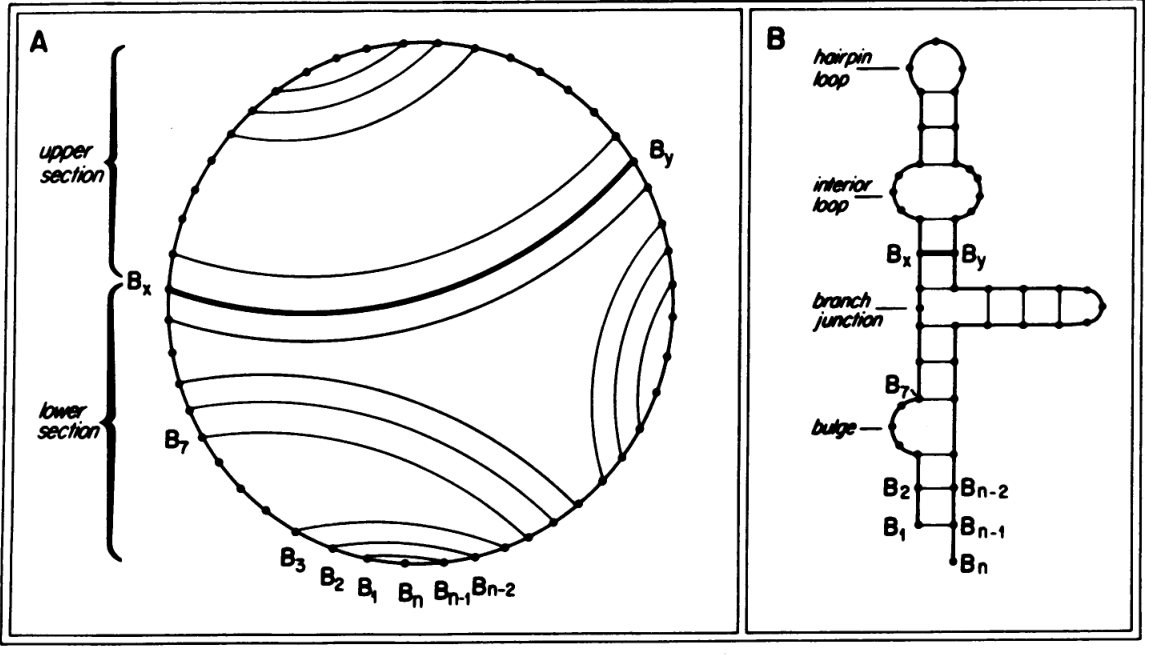
\includegraphics{figure1}}
\end{center}
\caption{RNA secondary structure as described in the Nussinov algorithm.
Taken from a publication by Nussinov \& Jacobson \cite{nussinov1980fast}.}
\label{nuss_rna}
\end{figure}


Because of its dynamic programming nature, this algorithm performs recursive decompositions of a RNA and builds
larger structures out of repeated substructures. A natural representation of this is
depicted in Figure \ref{nuss_rna}. Part A of Figure \ref{nuss_rna} shows bonds as arcs across a circular
graph. One can also see the nested nature of the structures being explored by the
Nussinov algorithm. Part B shows how these structures translate to actual RNAs,
and how they appear in vivo.

%you cant have several aligned equations in the same block
%unless you install a special package
%I have faked it here

\begin{equation} \label{eq:nuss_eq}
	M(i, j) = \max \left\lbrace A, B, C, D \right\rbrace
\end{equation}
\[
A = M(i, j-1)
\]
\[
B = M(i+1, j)
\]
\[
C = M(i+1, j-1) + W(i, j)
\]
\[
D = \max \left\lbrace M(i, k) + M(k+1, j) \right\rbrace \: when \: i < k < j
\]


Equation \ref{eq:nuss_eq} describes the recurrence relation for the Nussinov algorithm. The first two cases ($A$ and $B$) find the score associated with not allowing the positions $i$ and $j$ to bond. The case $C$ conversely determines the score, given that positions $i$ and $j$ are bonded. The final case $D$ computes the scores associated with bifurcations. A bifurcation here means decomposition of the RNA into two separate structures.


\subsection{The Zuker Algorithm}
Soon after the work of Nussinov \& Jacobson, Zuker \& Stiegler \cite{zuker1981optimal}
described an altered version of the same algorithm which, instead of maximising
bond weights, minimized free energy. This was done
by introducing a number of thermodynamic rules for canonical structures like
hairpin loops, internal bulges, multiloops, unbonded bases, and stacked base
pairs. The algorithm is similar to the Nussinov algorithm,
but requires another mutually recursive dynamic programming recurrence to inject
a complex and relatively comprehensive thermodynamic scoring system.


\begin{figure}
\begin{center}
\scalebox{0.27}{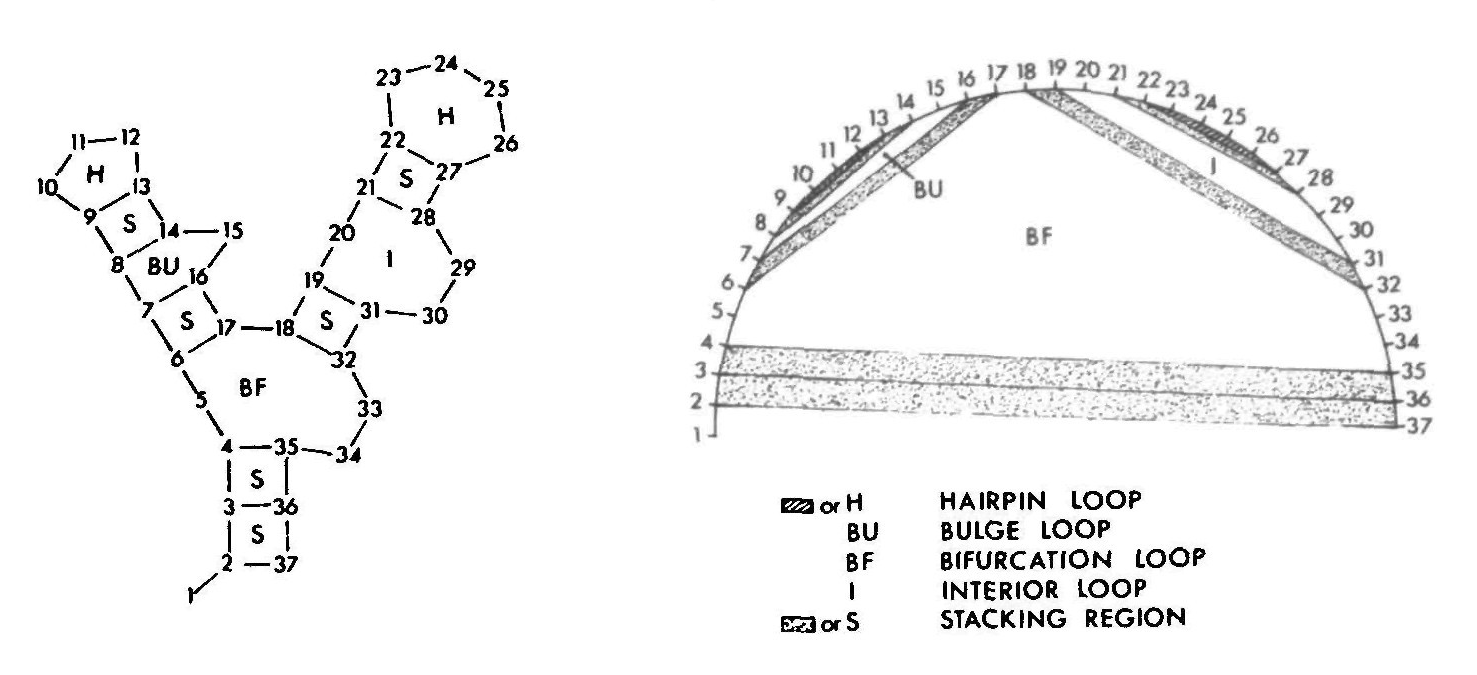
\includegraphics{figure4}}
\end{center}
\caption{Diagram of faces used in the Zuker algorithm. Taken from original
publication \cite{zuker1981optimal}.}
\label{zuk_struct}
\end{figure}

First I shall introduce some useful terminology which should clarify aspects of Zuker \& Stiegler’s
algorithm. The bases of a RNA molecule can be thought of as vertices in a planar graph. Edges between such vertices are then represented as chords on a semicircular diagram (see Figures \ref{nuss_rna} and \ref{zuk_struct}). These chords are not allowed to touch. A chord
is admissible if it represents a chemically valid bond, and an
admissible structure is a structure whose graph contains only admissible bonds.
Thence, one can define a face of such a graph as any planar region bounded on all
sides. The
folding algorithm of Zuker \& Stiegler considers such faces as the basic contributing factor to a molecule's stability, unlike the algorithm of Nussinov \& Jacobson
which considers only individual bonds.


Let $E(F)$ represent the energy of a face $F$; inadmissible structures are given
an energy value of infinity. In addition let $V(i, j)$ be defined as the minimum free
energy of all structures in which bases $i$ and $j$ are bonded, and let $W(i, j)$ represent
the minimum free energy of all structures contained within bases $i$ and $j$ inclusive.
Note that for $W(i, j)$ the bases at $i$ and $j$ need not be bonded. Alternatively if $i$ and $j$ cannot bond, then $V(i, j) = \infty $. Finally note that $FH(i, j)$ represents a
hairpin loop from $i$ to $j$, and that $FL(i, j, i' , j' )$ is defined as the region
bounded by the bonds $i, j$ and $i', j'$. Examples of these decompositions are shown
diagrammatically in the right half of Figure \ref{zuk_struct}. In the accompanying left
half the same RNA structure is shown as it would appear in vivo.

\begin{equation} \label{eq:zuk_v1_eq}
V(i, j) = \min \left\lbrace E1, E2, E3 \right\rbrace
\end{equation}
$$E1 = E(FH(i, j))$$
$$E2 = \min \left\lbrace E(FL(i, j, i', j')) + V (i', j') \right\rbrace \: where \: i < i' < j' < j$$
$$E3 = \min \left\lbrace W (i + 1, i') + W (i' + 1, j - 1) \right\rbrace \: where \: i + 1 < i' < j - 2$$


As defined in Equation \ref{eq:zuk_v1_eq}, $V (i, j)$ is computed by minimizing
three cases. The first case considers the bond between $i$ and $j$ closing off a hairpin
loop (H in Figure \ref{zuk_struct}). The second accounts for situations in which $i$ and $j$ are bonded, resulting in a bulge (BU in Figure \ref{zuk_struct}), internal loop (I in Figure \ref{zuk_struct}), or the continuation of a stacking region with the
interior bond $i',j'$ (S in Figure \ref{zuk_struct}). The third and final case considers bifurcations
(BF in Figure \ref{zuk_struct}).

\begin{equation} \label{eq:zuk_v1_eq2}
W (i, j) = \min \left\lbrace W(i + 1, j), W(i, j - 1), V(i, j), E4 \right\rbrace
\end{equation}
$$
E4 = \min \left\lbrace W (i, i') + W (i' + 1, j) \right\rbrace \: where \: i < i' < j - 1
$$

Equation \ref{eq:zuk_v1_eq2} is the recurrence for $W(i, j)$ as described by Zuker \& Stiegler.
Again there are three cases. The first two cases $W (i + 1, j)$ and $W(i, j - 1)$ are conceptually a single scenario in which there is no bond between $i$ and $j$. This is similar to cases $A$ and $B$ from the Nussinov algorithm (Equation \ref{eq:nuss_eq}). The third case considers taking the bond from
$i$ to $j$. The final case allows for bifurcations. The minimum free energy of the best structure is defined by $W(1, n)$, where $n$ is the length of the RNA molecule. It should
be noted that the free energy for small molecules (fewer than 6 nucleotides in length) can easily be
precomputed, and forms the base case of the given recurrence relations. Because of
its efficiency ($O(N^3)$ time and $O(N^2)$ space), robustness, and extensibility, this method is,
even today, still the most popular available. The most widely used packages for RNA secondary structure prediction all contain implementations of the Zuker algorithm \cite{lorenz2011viennarna, reuter2010rnastructure}.


\section{Stochastic Context Free Grammars}

Later, in the early 90s, Hidden Markov models and Stochastic Context Free Grammars (SCFGs) were being used to model RNA folding. Sakakibara et al. \cite{sakakibara1994stochastic} used SCFGs to accurately fold tRNAs, a family of RNAs with notoriously difficult to predict secondary structures. They did this by defining a formal grammar that parsed secondary structure elements into the original primary sequence, with probabilities assigned to the production rules. These probabilities can be trained using actual RNAs, yielding a model capable of parsing novel RNA sequences. Later methods were similar, but worked for general classes of RNAs \cite{dowell2004evaluation, knudsen2003pfold}.

In 2012 Rivas, Lang \& Eddy \cite{rivas2012range} presented a computation tool called TORNADO which can parse various RNA grammars. It supports the typical grammars used in SCFG approaches, the grammar implicit in Zuker's algorithm upon which the thermodynamic model is based, and many more complex grammars. They used this meta-algorithm to compare the current state of the art models. Because TORNADO is essentially a super-SCFG parser, all of the supported grammars can have their parameters changed arbitrarily. Hence, the experimentally determined thermodynamic model, which the Zuker algorithm uses, can be applied to other grammars, and complex, machined learned parameters can be applied to the Zuker grammar. Rivas, Lang \& Eddy found that the best machine learned models are comparable to the typical thermodynamic model in accuracy, however they often suffered from overfitting.

\subsection{Unification of Techniques}

In a subsequent publication, Rivas \cite{rivas2013four} unified pseudoknot-free RNA folding algorithms. Her core observation is that all such prediction algorithms contain the same four key components: an architecture, or the production rules of a grammar; a scoring scheme, or how scores are assigned to these production rules; and the parametrization of the scoring scheme, or the specific values assigned to it. These three features are referred to by Rivas as the `model'. The fourth and final feature is the folding algorithm used to find the best structure given the model. Here Rivas notes that the two dominant folding algorithms are interchangeable. The Cocke-Younger-Kasami (CYK) algorithm used to parse SCFGs and algorithms based on the work of Zuker \& Stiegler are isomorphic for the purpose of parsing RNA grammars. Rivas additionally notes that all scoring schemes and parametrizations appear to hit an accuracy upper limit, and that complex, machine learned models are only slightly more accurate than thermodynamic models. In fact, relatively basic grammars with hundreds of parameters seem to perform almost equivalently to those with tens of thousands.

\begin{figure}
\begin{center}
\scalebox{0.27}{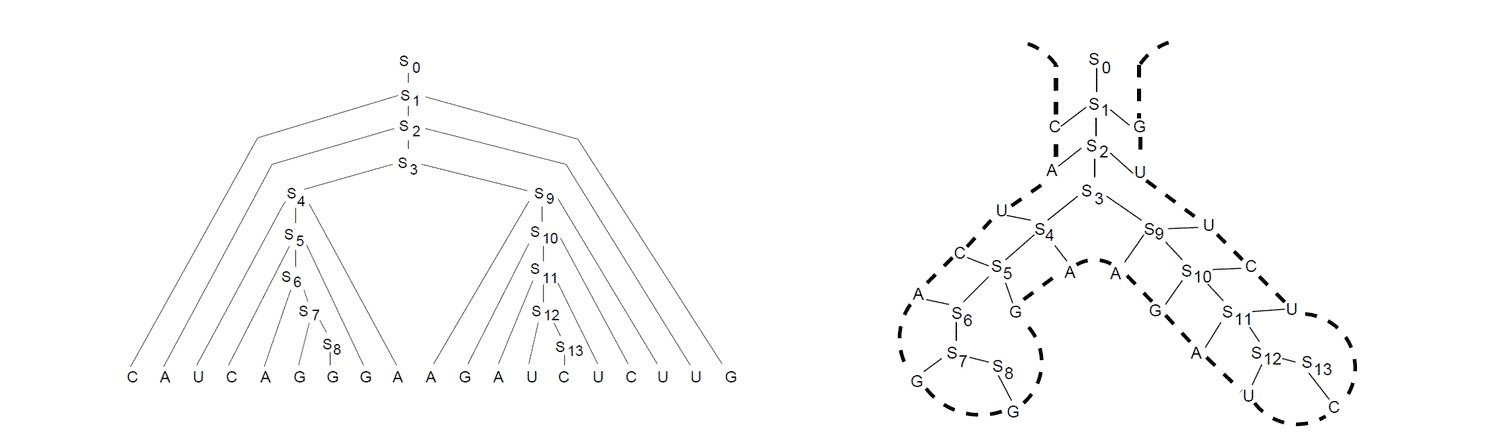
\includegraphics{scfg}}
\end{center}
\caption{Left shows the parse tree for a context free grammar. Right shows how this tree relates to RNA secondary structure. Taken from original publication \cite{sakakibara1994stochastic}.}
\label{fig:scfg}
\end{figure}


\section{Conclusions}
Current state of the art algorithms fold RNA in a way that globally maximises their score according to some model. The Zuker algorithm, for example, finds the global minimum free energy configuration. SCFGs globally maximise the perceived probability according to some grammar. This bias is largely due to the Thermodynamic Hypothesis. Anfinsen \cite{anfinsen1973principles} presented this hypothesis as the underlying principle behind the formation of biologically active proteins. He held that protein fold into the minimum Gibbs free energy conformation in their typical biological environment; environment being defined as the molecules' physiological state: pH, temperature, and ion concentration. Furthermore, through natural selection, molecules that are most likely to fold into the correct shape have evolved, and the atomic interactions of such molecules fully determine their final state. This insight has been invaluable for folding proteins and RNAs in silico. Despite this, it has recently become clear that methods for the prediction of RNA secondary structures have hit an upper limit in accuracy.

Perhaps the Thermodynamic Hypothesis is insufficiently powerful to explain in vivo RNA secondary structures. As Rivas \cite{rivas2013four} noted, there appears to be a ceiling on the accuracy of our current algorithms; which are based on the Thermodynamic Hypothesis. Finding a way beyond this barrier will be important for future advancements, as it is increasingly obvious that RNAs are essential biological agents. RNA prediction is a liminal field, and in dire need of a way beyond the Thermodynamic Hypothesis.





%let bibtex do all the hard work
\bibliographystyle{plain}
\bibliography{assignment_two}


\end{document}

